% This is the template for the standard non-english version of the journal article at the Journal of Artificial Intelligence for Sustainable Development (JAISD) https://www.jaisd.org/

% The Journal of Artificial Intelligence for Sustainable Development (JAISD) serves as a critical platform to examine the ethical dimensions of AI and propose responsible, equitable, and impactful solutions to advance the UN SDGs. We curate and publish high-quality, peer-reviewed research on topics such as algorithmic fairness, transparency, accountability, environmental impact, and the intersection of technological innovation and societal well-being.

% letterpaper/a4paper: US/UK paper size toggle
% num-refs/alpha-refs: numeric/author-year citation and bibliography toggle

\documentclass[a4paper,alpha-refs]{jaisd}

\usepackage{graphicx}
\usepackage{siunitx}
\usepackage{lipsum}
\usepackage{caption}
\usepackage{lipsum}
\usepackage{float}
\captionsetup{justification=centering} 

% To submit a version in other language than french, please change title as appropriate 
\renewcommand{\abstractname}{Résumé}

%%% Flushend: You can add this package to automatically balance the final page, but if things go awry (e.g. section contents appearing out-of-order or entire blocks or paragraphs are coloured), remove it!
% \usepackage{flushend}

%%% Paper category
% To submit a version in other language than french, please change title as appropriate 
\papercat{Document de Position}

\title{Titre du Document de Recherche}

%%% Use the \authfn to add symbols for additional footnotes, if any. 1 is reserved for correspondence emails; then continuing with 2 etc for contributions.
\author[1,2,\authfn{1}]{author1}
\author[3,\authfn{2}]{author2}
%\author[2]{Third Author}
%\author[2,\authfn{1}]{Fourth Author}

\affil[1]{affiliation1, location}
\affil[2]{affiliation1, location}
\affil[3]{affiliation1, location}

%%% Author Notes
\authnote{\authfn{1}email@author1}
\authnote{\authfn{2}email@author2}

%%% "Short" author for running page header
\runningauthor{Author1 et al.}

%%% Should only be set by an editor
\jvolume{1}
\jnumber{1}
\jyear{2024}
\jstartpage{8}
\setcounter{page}{8}
\jdoi{10.69828/4d4ke6}

\begin{document}

\begin{frontmatter}
\maketitle
\begin{abstract}
\lipsum[1]
\medskip

\textit{Mots-clés: keyword1, keyword2, keyword3, keyword4, keyword5}
%
\end{abstract}

\end{frontmatter}

\section{Introduction}
\lipsum[2] \cite{UNESCO21}

\section{Section}
\lipsum[3] \cite{Lukowicz23}

\section{Section}
\lipsum[4] \cite{DeepMind18}

\begin{table}[H]
\begin{tabularx}{\textwidth}{CCC}
\toprule
\textbf{Title 1}	& \textbf{Title 2}	& \textbf{Title 3}\\
\midrule
Entry 1		& Data			& Data\\
Entry 2		& Data			& Data\\
\bottomrule
\end{tabularx}
\caption{This is a table caption.}
\label{tab5}
\end{table}

\begin{figure}[H]
  \centering
    \captionsetup{type=figure}
    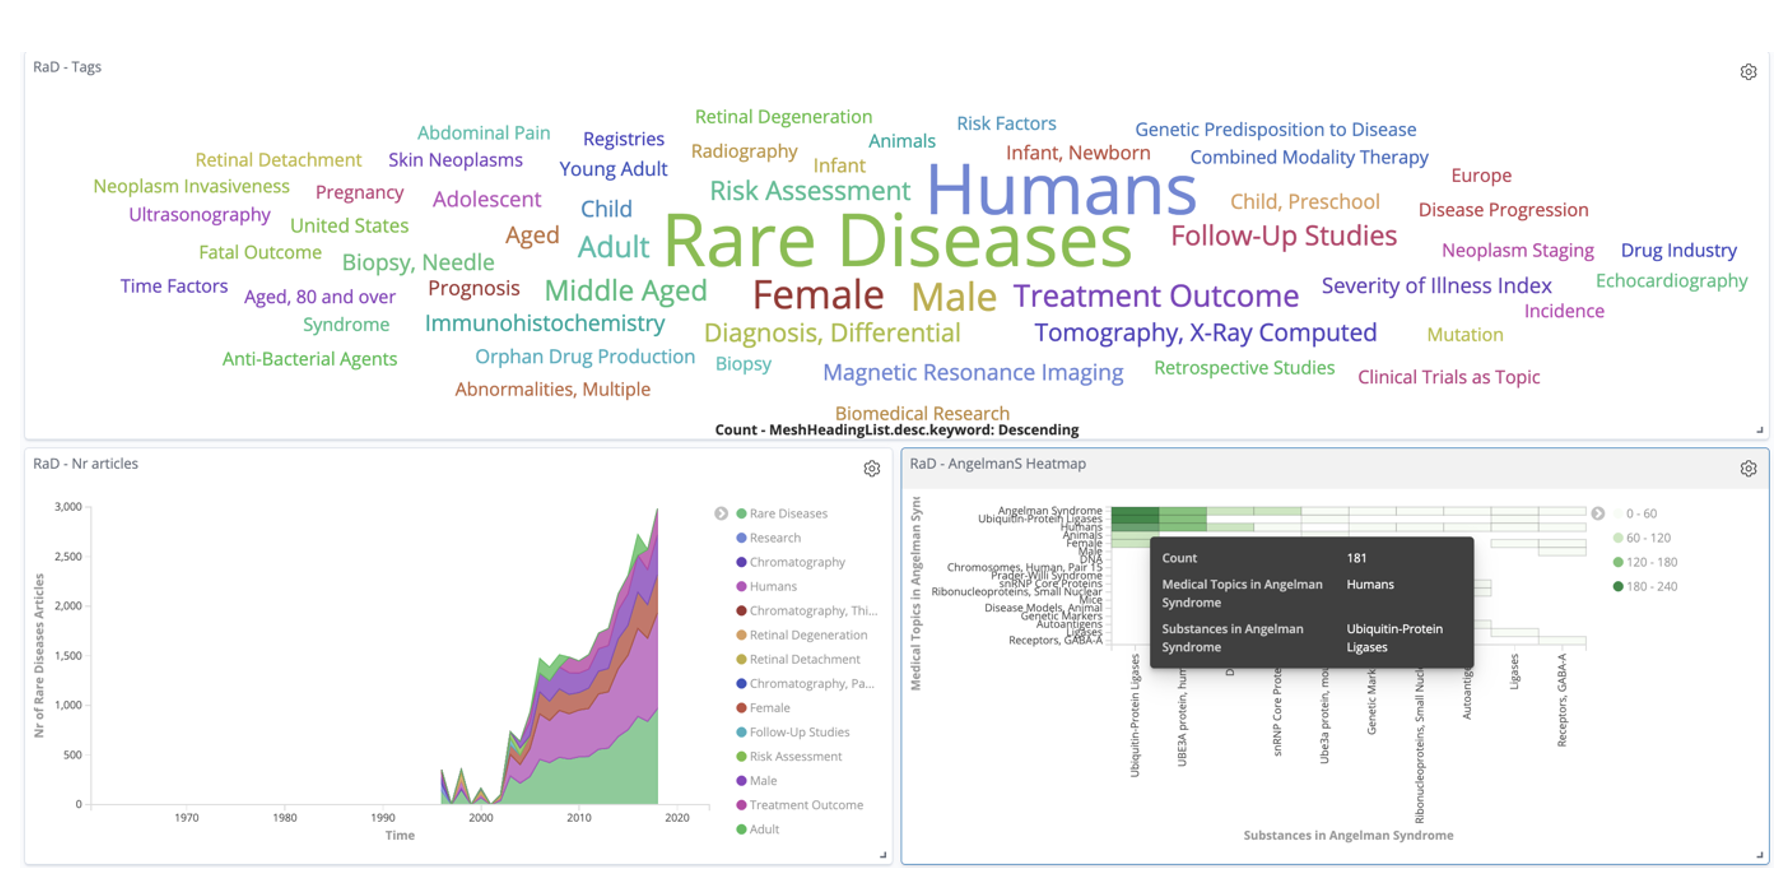
\includegraphics[width=0.85\linewidth]{fig3.png}
    \captionof{figure}{This is the caption of the figure.}
    \label{fig:fig3}
    \vspace{-0.1cm}
\end{figure}

% To submit a version in other language than french, please change title as appropriate 
\subsection{Financement}

Ce travail est partiellement soutenu par ...

% To submit a version in other language than french, please change title as appropriate 
\subsection{Contribution de l'auteur}

\lipsum[5]

% To submit a version in other language than french, please change title as appropriate 
\section{Remerciements}

%\subsection{Data Access}  % to define the access to the data used, if applicable

\lipsum[6] 

%% Specify your .bib file name here, without the extension
\bibliography{paper-refs}

\end{document}
